\onecolumn
\chapter{Auswertung}
\label{ch:auswertung}

\section*{Fehlerrechnung}
Für die statistische Auswertung von $n$ Messwerten $x_i$ werden folgende Größen definiert \cite{errorSkript25}:
\begin{align}
    \bar{x} &= \frac{1}{n} \sum_{i=1}^{n} x_i \vphantom{\sqrt{\sum_i^n}^2} && \text{\textcolor{gray}{Arithmetisches Mittel}} \label{eq:arithmetisches_mittel} \\
    \sigma^2 &= \frac{1}{n-1} \sum_{i=1}^{n} (x_i - \bar{x})^2 \vphantom{\sqrt{\sum_i^n}^2} && \text{\textcolor{gray}{Variation}} \label{eq:variation} \\
    \sigma &= \sqrt{\frac{1}{n-1} \sum_{i=1}^{n} (x_i - \bar{x})^2} \vphantom{\sqrt{\sum_i^n}^2} && \text{\textcolor{gray}{Standardabweichung}} \label{eq:standardabweichung} \\
    \Delta \bar{x} &= \frac{\sigma}{\sqrt{n}} = \sqrt{\frac{1}{n(n-1)} \sum_{i=1}^n(\bar x - x_i)^2} \vphantom{\sqrt{\sum_i^n}^2} && \text{\textcolor{gray}{Fehler des Mittelwerts}} \label{eq:fehler_mittelwert} \\
    \Delta f &= \sqrt{\left(\frac{\partial f}{\partial x} \Delta x\right)^2 + \left(\frac{\partial f}{\partial y} \Delta y\right)^2} \vphantom{\sqrt{\sum_i^n}^2} && \text{\textcolor{gray}{Gauß’sches Fehlerfortpflanzungsgesetz für $f(x,y)$}} \label{eq:gauss_fehlfortpflanzung} \\
    \Delta f &= \sqrt{(\Delta x)^2 + (\Delta y)^2} \vphantom{\sqrt{\sum_i^n}^2} && \text{\textcolor{gray}{Fehler für $f = x + y$}} \label{eq:fehler_summe} \\
    \Delta f &= |a| \Delta x \vphantom{\sqrt{\sum_i^n}^2} && \text{\textcolor{gray}{Fehler für $f = ax$}} \label{eq:fehler_proportional} \\
    \frac{\Delta f}{|f|} &= \sqrt{\left(\frac{\Delta x}{x}\right)^2 + \left(\frac{\Delta y}{y}\right)^2} \vphantom{\sqrt{\sum_i^n}^2} && \text{\textcolor{gray}{relativer Fehler für $f = xy$ oder $f = x/y$}} \label{eq:relativer_fehler} \\
    \sigma &= \frac{|a_{lit} - a_{gem}|}{\sqrt{\Delta a_{lit}^2 + \Delta a_{gem}^2}} \vphantom{\sqrt{\sum_i^n}^2} && \text{\textcolor{gray}{Berechnung der signifikanten Abweichung}} \label{eq:signifikante_abweichung}
\end{align}

\twocolumn
\section{Bestimmung der theoretischen Schallgeschwindigkeit}
Es soll die Schallgeschwindigkeit in Luft und Kohlenstoffdioxid bei den im Versuch herrschenden Bedingungen bestimmt werden. Dazu wird \hyperref[eq:theorie_c]{Gleichung~\ref*{eq:theorie_c}} verwendet. Die Adiabatenkoeffizienten von Liuft und Kohlenstoffdioxid sind dem Skript \cite{skript25} entnommen und betragen:
\begin{align}
    \kappa_{Luft} &= 1,4 \\
    \kappa_{CO_2} &= 1,3
\end{align}

Die molaren Massen ergeben sich aus den Atomgewichten der beteiligten Elemente:
\begin{align}
    M_{Luft} &= 29\,\frac{g}{mol} \\
    M_{CO_2} &= 44\,\frac{g}{mol}
\end{align}

R ist die ideale Gaskonstante mit $R = 8,314\,\frac{J}{mol\,K}$. Die Temperatur wird auf den Idealwert von $T = 273,15\,K$ (0°C) bestimmt. Damit ergeben sich die theoretischen Schallgeschwindigkeiten zu:
\begin{equation}
    \boxed{
        c_{Luft} = 331,11\,\frac{m}{s} \\
    }
\end{equation}
        
\begin{equation}
    \boxed{
        c_{CO_2} = 259,03\,\frac{m}{s}
    }
\end{equation}
    
Das Verhältnis der Schallgeschwindigkeiten beträgt:
\begin{equation}
    \boxed{
        \frac{c_{Luft}}{c_{CO_2}} = 1,278
    }
    \label{eq:theorie_verhaeltnis}
\end{equation}

\section{Bestimmung der Schallgeschwindigkeit mit dem Quincke'schen Rohr}
Die Messdaten für die Bestimmung der Schallgeschwindigkeit mit dem Quincke'schen Rohr sind den Tabellen 1 (Luft) und 2 (Kohlenstoffdioxid) des \hyperref[Protokoll]{Protokolls} zu entnehmen. Die Frequenz des Generators beträgt $(\nu = 21\,000 \pm 0,5)\,Hz$. Über diese soll die Schallgeschwindigkeit in den beiden Medien bestimmt werden. Dazu werden außerdem die Abstände zwischen aufeinanderfolgenden Resonanzstellen benötigt. Mit dieser wird die Wellenlänge über \hyperref[eq:wellenlaenge]{Gleichung~\ref*{eq:wellenlaenge}} bestimmt, welche nachfolgend als $d$ bezeichnet wird. Die Schallgeschwindigkeit ergibt sich dann über \hyperref[eq:c_aus_lambda]{Gleichung~\ref*{eq:c_aus_lambda}}. 
Die Ungenauigkeit der Differenz wird über die \hyperref[eq:gauss_fehlfortpflanzung]{Gauß'sche Fehlerfortpflanzung (\ref*{eq:gauss_fehlfortpflanzung})} bstimmt:
\begin{equation}
    \Delta d_{sys} = 2 \cdot \sqrt{(\Delta h_{i+1})^2 + (\Delta h_i)^2}.
\end{equation}
Die Ablesegenauigkeit wird auf $\Delta h = 0,25\,cm$ geschätzt.

Dazu wird die statistische Ungenauigkeit $d_{stat}$ über die \hyperref[eq:fehler_mittelwert]{Standardabweichung des Mittelwerts (\ref*{eq:fehler_mittelwert})} bestimmt.

Der gesamte Fehler der Differenz ergibt sich dann über:
\begin{equation}
    \Delta d = \sqrt{(\Delta d_{sys})^2 + (\Delta d_{stat})^2}.
\end{equation}

Daraus lässt sich die Ungenauigkeit der Wellenlänge bestimmen:
\begin{equation}
    \Delta \lambda = 2 \cdot \Delta d.
\end{equation}

Die Unsicherheit der Schallgeschwindigkeit ergibt sich ebenfalls über die Gauß'sche Fehlerfortpflanzung:
\begin{equation}
    \Delta c = \sqrt{(\nu \cdot \Delta \lambda )^2 + (\lambda \cdot \Delta \nu)^2}.  
\end{equation}

Die gemessene Raumtemperatur beträgt $T_{gem} = (23,0 \pm 1,0)^\circ C = (296,2 \pm 1,0)\,K$. Mit dieser wird die Schallgeschwindigkeit auf Normalbedingungen umgerechnet. Dazu wird \hyperref[eq:normbedingungen]{Gleichung~\ref*{eq:normbedingungen}} verwendet, wobei $T_0 = 273,15\,K$ die Normaltemperatur ist. Die Unsicherheit der Schallgeschwindigkeit bei Normalbedingungen wird über die Gauß'sche Fehlerfortpflanzung bestimmt:
\begin{equation}
    \Delta c_0 = \sqrt{\left( \frac{\Delta T}{2T} \right)^2 + \left(\frac{\Delta c}{c}\right)^2} \, \cdot c_0.
\end{equation}   

Aus den zwei Messreihen wird das \hyperref[eq:arithmetisches_mittel]{arithmetische Mittel (\ref*{eq:arithmetisches_mittel})} bestimmt. Zwischen diesen Einträgen werden die Differenzen gebildet, um die Wellenlänge zu bestimmen. Ausdiesen Werten wird wiederum das arithmetische Mittel gebildet und sein Fehler bestimmt. 

\subsection{Luft}
Für die die durchschnittliche Differenz zwischen aufeinanderfolgenden Resonanzstellen ergibt sich:
\begin{equation}
    \underline{
        \overline{d_{Luft}} = (8,2 \pm 0,8)\,cm.
    }
\end{equation}

Und damit die Wellenlänge:
\begin{equation}
    \underline{
        {\lambda_{Luft}} = (16,5 \pm 1,5)\,cm.
    }
\end{equation}

Damit lässt sich die Schallgeschwindigkeit der gegebenen Umstände bestimmen. Diese kommt auf einen Wert von:
\begin{equation}
    \boxed{
        c_{Luft} = (350 \pm 30) \frac{m}{s}
    }
\end{equation}

Die Hohe Ungenauigkeit hängt mit dem großen Ablehsefehler zusammen. Ohne Ablese Fehler käme man auf ein Ergebnis von:
\begin{equation}
\underline{c_{Luft,2} = (345,9 \pm 11,7)}.
\end{equation}

Die Schallgeschwindigkeit unter Normalbedingungen beläuft sich somit auf:
\begin{equation}
\boxed{
    c_{0,Luft} = (360 \pm 30) \, \frac{m}{s}
}
\end{equation}

Wieder ohne Ablesefehler:
\begin{equation}
\underline{
    c_{0,Luft,2} = (360,1677 \pm 12,1228) \, \frac{m}{s}
}
\end{equation}

\subsection{Kohlenstoffdioxid}
Analog wird die Schallgeschwindigkeit im Kohlenstoffdioxid bestimmt. Die Durchschnittsdifferenz beträgt dabei
\begin{equation}
    \underline{
        \overline{d_{CO_2}} = (6,4 \pm 0,7) \, \mathrm{cm},
    }
\end{equation}
aus der sich die Wellenlänge
\begin{equation}
    \underline{\lambda_{CO_2} = (12,9 \pm 1,4)}.
\end{equation}
berechnet.

Somit beträgt die Schallgeschwindigkeit in Kohlenstoffdioxid
\begin{equation}
\boxed{
    c_{CO_2} = (271,0 \pm 30,0) \, \mathrm{\frac{m}{s}}
}
\end{equation}

und unter Normalbedingungen:
\begin{equation}
\boxed{
    c_{0,CO_2} = (280 \pm 30) \, \mathrm{\frac{m}{s}}
}
\end{equation}

Unter Vernachlässigung der Ableseungenauigkeit kommen die Ergbenisse: 
\begin{equation}
\underline{
    c_{CO_2,2} = (270,6\pm 0,9)  \, \mathrm{\frac{m}{s}}
    }
\end{equation}
und
\begin{equation}
\underline{
    c_{0,CO_2,2} = (281,7341\pm 1,0205) \, \mathrm{\frac{m}{s}}
    }
\end{equation}

\subsection{Signifikanz}
Die Werte sollen \hyperref[tab:ergbnisse_1]{tabellarisch \ref*{tab:ergbnisse_1}} aufgelstet werden und deren \hyperref[eq:signifikante_abweichung]{Berechnung der signifikanten Abweichung (\ref*{eq:signifikante_abweichung})} soll bestimmt werden.
\begin{table}[!ht]
    \centering
    \begin{tabular}{c | c | c}
        \toprule
        Größe & Luft & $CO_2$ \\
        \hline
        d [cm] & $8,2 \pm 0,8$ & $6,4 \pm 0,7$ \\
        $\lambda$ [cm] & $16,5 \pm 1,5$ & $12,9 \pm 1,4$ \\ 
        \midrule
        c [m/s] & $350 \pm 30$ & $271,0 \pm 30,0$ \\
        $c_0$ [m/s] & $360 \pm 30$ & $280 \pm 30$ \\
        \midrule
        $c_2$ [m/s] & $345,9 \pm 11,7$ & $270,6 \pm 0,9$ \\
        $c_{0,2}$ [m/s] & $360,1677 \pm 12,1228$ & $281,7341 \pm 1,0205$ \\
        \midrule
        \midrule
        $\sigma$ & $0,31\sigma$ & $0,24\sigma$ \\
        $\sigma_2$ & $0,28\sigma$ & $8,40\sigma$ \\
        \bottomrule
    \end{tabular}
    \label{tab:ergbnisse_1}
    \caption{Zusammenfassung der Ergebnisse aus der Quinche'schen Röhre.}
\end{table}

Die >>2<< indiziert dabei die ausschließliche Nutzung des statistischen Fehlers, der systematische Ablesefehler wird somit nicht berücksichtigt.

\subsection{Verhältnis der Schallgeschwindigkeiten}
Zuletzt soll das Verhältnis der Schallgeschwindigkeiten in Luft und Kohlenstoffdioxid bestimmt werden. Das Verhältnis beträgt: 
\begin{equation}
\frac{c_{0,Luft}}{c_{0,CO_2}}.
\end{equation}

Über die \hyperref[eq:gauss_fehlfortpflanzung]{Gauß'sche Fehlerfortpflanzung (\ref*{eq:gauss_fehlfortpflanzung})} wird der Fehler zu
\begin{equation}
    \Delta \left(\frac{c_{0,L}}{c_{0,CO_2}}\right) = \sqrt{\left(\frac{\Delta c_{0,L}}{c_{0,CO_2}}\right)^2 + \left(\frac{c_{0,L} \cdot \Delta c_{0,CO_2}}{{c_{0,CO_2}}^2}\right)^2}
\end{equation}
bestimmt.

Somit Ergibt sich für das Verhältnis:
\begin{equation}
    \boxed{
        \frac{c_{0,Luft}}{c_{0,CO_2}} = 1,29 \pm 0,17
    }.
\end{equation}

Die entspricht einer \hyperref[eq:signifikante_abweichung]{signifikanten Abweichung (\ref*{eq:signifikante_abweichung})} von:
\begin{equation}
    \sigma = 0,07\sigma
\end{equation}
Zum bestimmten \hyperref[eq:theorie_verhaeltnis]{Theoriewert \ref*{eq:theorie_verhaeltnis}}.

Nutzt man die Werte ohne Ablesefehler, so ergibt sich
\begin{equation}
    {
        \frac{c_{0,Luft,2}}{c_{0,CO_2,2}} = 1,28 \pm 0,04
    },
\end{equation}
und eine signifikante Abweichung von
\begin{equation}
    \sigma_2 = 0,05\sigma
\end{equation}
Zum bestimmten \hyperref[eq:theorie_verhaeltnis]{Theoriewert \ref*{eq:theorie_verhaeltnis}}.

\section{Bestimmung der Schallgeschwindigkeit via Laufzeitmessung}
Es soll nun der Versuchsaufbau mit dem Osziloskop betrchtet werden. Hier sind zwei Messreihen durchgeführt worden. Beide im Luft-Medium, jedoch mit unterschiedlichen Osziloskopeinstellungen. Die Messdaten sind den Tabellen 3 und 4 des \hyperref[Protokoll]{Protokolls} zu entnehmen. Tabelle 3 beinhaltet die Messwerte des Osioloskopes unter benutzung des Y-t Moduses, also der Verschiebung des Signals über die Zeitachse. Tabelle 4 beinhaltet die Messwerte des Osziloskopes unter benutzung des X-Y Moduses.
Beide Modi sollen mit einander verglichen werden.

\subsection{Y-t Modus}
\begin{figure}[!ht]
    \centering
    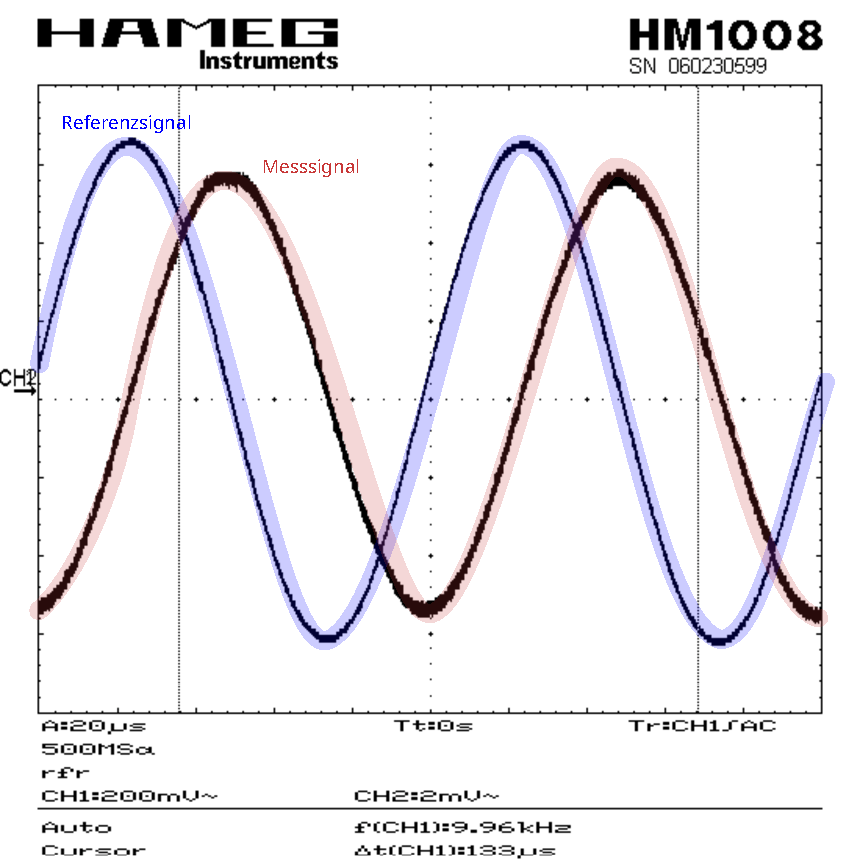
\includegraphics[width=0.45\textwidth]{img/26/SinusRef.pdf}
    \caption{Beispiel eines Messwertes im Y-t-Modus bei 10kHz.}
    \label{fig:yt_modus}
\end{figure}

Die \hyperref[ig:yt_modus]{Abbildung \ref*{fig:yt_modus}} zeigt ein Beispiel eines Messwertes im Y-t Modus. Hier ist die Verschiebung des Signals über die Zeitachse abgebildet. Die Frequenz des Generators beträgt $\nu = 10\,kHz$. Die Zeitdifferenz zwischen den beiden Signalen wird abgelesen und in eine Wegstrecke umgerechnet. 
Es wurden wieder jeweils zwei Messreihen vorgenommen, um die statistische Genauigkeit zu erhöhen. Es werden wieder die Differenzen zwischen aufeinanderfolgenden Messwerten gebildet, um die Wellenlänge zu bestimmen. Aus diesen Werten wird wiederum das arithmetische Mittel gebildet und sein Fehler bestimmt. Der Fehler berechnet sich aus dem systematischen Ablesefehler von $\Delta d = 0,5\,cm$ und dem \hyperref[eq:fehler_mittelwert]{Fehler des Mittelwerts (\ref*{eq:fehler_mittelwert})}. Folglich ergibt sich für die erste Messreihe eine Wellenlänge von:
\begin{equation}
    \underline{
        \lambda_1 = (3,5 \pm 0,5)\,cm
    }
\end{equation}

Mit der Frequenz von $\nu = 10\,kHz$ ergibt sich eine Schallgeschwindigkeit von:
\begin{equation}
    \boxed{
        c_1 = (350 \pm 50)\,\frac{m}{s}
    }
\end{equation}

Unter Normalbedingungen:
\begin{equation}
    \boxed{
        c_{0,1} = (360 \pm 60)\,\frac{m}{s}
    }
\end{equation}

\subsection{X-Y Modus}
\begin{figure}[!ht]
    \centering
    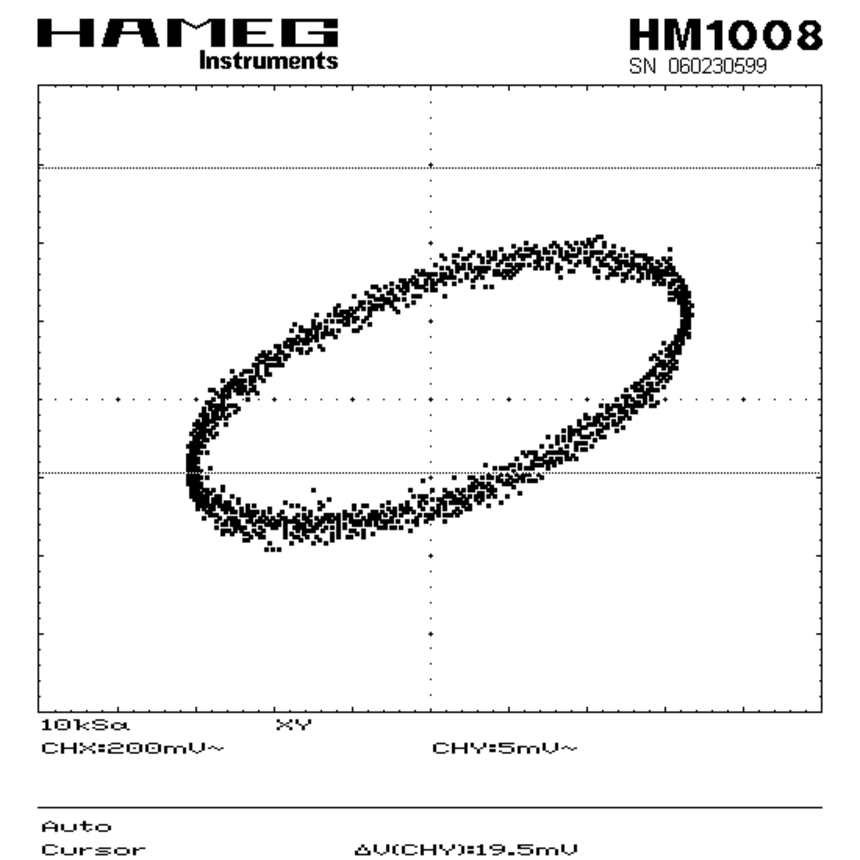
\includegraphics[width=0.45\textwidth]{img/26/YX.pdf}
    \caption{Beispiel eines Messwertes im X-Y-Modus bei 10kHz.}
    \label{fig:xy_modus}
\end{figure}

Die \hyperref[fig:xy_modus]{Abbildung \ref*{fig:xy_modus}} zeigt ein Beispiel eines Messwertes im X-Y Modus. Hier ist die Verschiebung des Signals über die X-Achse abgebildet. Die Frequenz des Generators beträgt $\nu = 10\,kHz$.

Die Wellenlänge bestimmt sich zu 
\begin{equation}
\underline{
    \lambda_2 = (3,4857 \pm 1,0006)\,cm
}
\end{equation}

Aus dieser Ergibt sich die Schallgeschwindigkeit zu:
\begin{equation}
\boxed{
    c_2 = (348,57 \pm 100,06)\,\frac{m}{s}
}
\end{equation}

Unter Normalbedingungen:
\begin{equation}
\boxed{
    c_{0,2} = (362 \pm 104)\,\frac{m}{s}
}
\end{equation}

\subsection{Vergleich der Modi}
Die Ergebnisse sollen im Folgendem verglichen werden. Die Bestimmung der Signifikanz unter benutzung dieser Werte ist jedoch nicht sinnvoll, da die Unsicherheiten durch den Ablesefehler sehr groß sind. Es fällt jedoch auf, dass die Ungenauigkeiten mit Ablesefehler im Y-t-Modus geringer sind als im X-Y-Modus. Dennoch sind die Werte mit Ableseungenauigkeit kaum aussagekräftig. Ohne Ablesefehler sind die Werte jedoch sehr genau und liegen nah beieinander. Die Ergebnisse sind in \hyperref[tab:vergleich_modus]{Tabelle \ref*{tab:vergleich_modus}} zusammengefasst.
\begin{table}[!ht]
    \centering
    \begin{tabular}{c | c | c}
        \toprule
        Größe & Y-t Modus & X-Y Modus \\
        \hline
        $\lambda$ [cm] & $3,5 \pm 0,5$ & $3,4857 \pm 1,0006$ \\
        \midrule
        c [m/s] & $350 \pm 50$ & $348,57 \pm 100,06$ \\
        $c_0$ [m/s] & $360 \pm 60$ & $362 \pm 104$ \\
        \midrule
        $c_2$ [m/s] & $349 \pm 18$ & $349 \pm 3$ \\
        $c_{0,2}$ [m/s] & $364 \pm 19$ & $363 \pm 4$ \\
        \bottomrule
    \end{tabular}
    \caption{Zusammenfassung der Ergebnisse aus dem Osziloskop.}
    \label{tab:vergleich_modus}
\end{table}

Es wird schnell ersichtlich, dass die Ergebnisse ohne Ablesefehler (Indizie >>2<<) genauer sind und näher beieinander liegen. Besonders die Ungenauigkeit im X-Y Modus ist hier sehr viel geringer im Vergleich. Die statistische Signifikanz der Ergebnisse ohne Ablesefehler beträgt:
\begin{equation}
    \sigma_2 = \frac{\left| c_{Y-t} - c_{Y-X} \right|}{\sqrt{(\Delta c_{Y-t})^2 + (\Delta c_{Y-t})^2}} = 0,04\sigma
\end{equation}

Eigentlich wäre die Abweichung null, da die Rundung jedoch unterschiedlich ist, ergibt sich eine kleine Abweichung. Diese ist jedoch nicht signifikant. Vergleichbar ist dies mit den Ergebnissen der Normalbedingungen
\begin{equation}
    \sigma_2 = \frac{\left| c_{0,Y-t} - c_{0,Y-X} \right|}{\sqrt{(\Delta c_{0,Y-t})^2 + (\Delta c_{0,Y-t})^2}} = 0,05\sigma
\end{equation}

\subsection{Gesamtvergleich}
Abschließend sollen die Ergebnisse der beiden Methoden verglichen werden. Auch hier ist die Signifikanz der Werte mit Ablesefehler nicht sinnvoll, da die Ungenauigkeiten zu groß sind. Ohne Ablesefehler ergeben sich jedoch folgende Werte. Es werde die Werte aus dem Y-X-Modus des Osziloskops verwendet, da diese die geringste Ungenauigkeit aufweisen. Somit ist die \hyperref[eq:signifikante_abweichung]{signifikante Abweichung (\ref*{eq:signifikante_abweichung})} zwischen den beiden Methoden:
\begin{equation}
    \sigma_2 = \frac{\left| c_{Quincke} - c_{Oszilloskop} \right|}{\sqrt{(\Delta c_{Quincke})^2 + (\Delta c_{Oszilloskop})^2}} = 0,26\sigma
\end{equation}
Für die Normalbedingungen beträgt die signifikante Abweichung:
\begin{equation}
    \sigma_2 = \frac{\left| c_{0,Quincke} - c_{0,Oszilloskop} \right|}{\sqrt{(\Delta c_{0,Quincke})^2 + (\Delta c_{0,Oszilloskop})^2}} = 0,22\sigma
\end{equation}

\section{Aufgenommene Stimme}
Die Stmme wurde mit dem Versuchsaufbau des Oszilloskops aufgenommen. Dabei wurde die Visuakisierung über den FFT-Modus vorgenommen. Die schönsten Ergebnisse sind unter Pfeifen entstanden, da diese eien spezifische Eigenfrequenz aufweisen und sich die Obertöne gut erkennen lassen. Dies sind die Frequenzen bei denen die Amplitude besonders hoch ist. 
\begin{figure}[!ht]
    \centering
    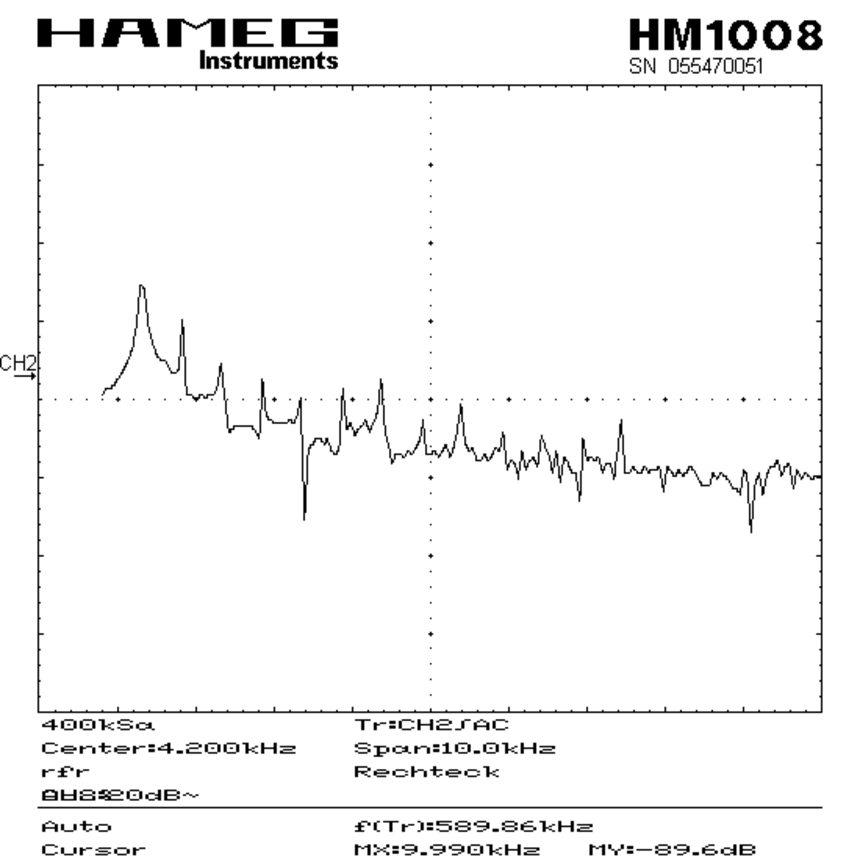
\includegraphics[width=0.45\textwidth]{img/26/Stimme.pdf}
    \caption{FFT der aufgenommenen Stimme (Pfeifen).}
    \label{fig:stimme_fft}
\end{figure}

\section{Invarianz der Frequenz}
Die genutze Frequenz des Generators hat keine Auswirkung auf die Schallgeschwindigkeit. Dies wurde qualitativ überprüft, indem die Frequenz des Generators auf 2kHz, 5kHz und 10kHz eingestellt wurde. Die Position der Resonanzstellen hat sich dabei nicht verändert. Dies bestätigt die Invarianz der Frequenz.
\begin{figure}[!ht]
    \centering
    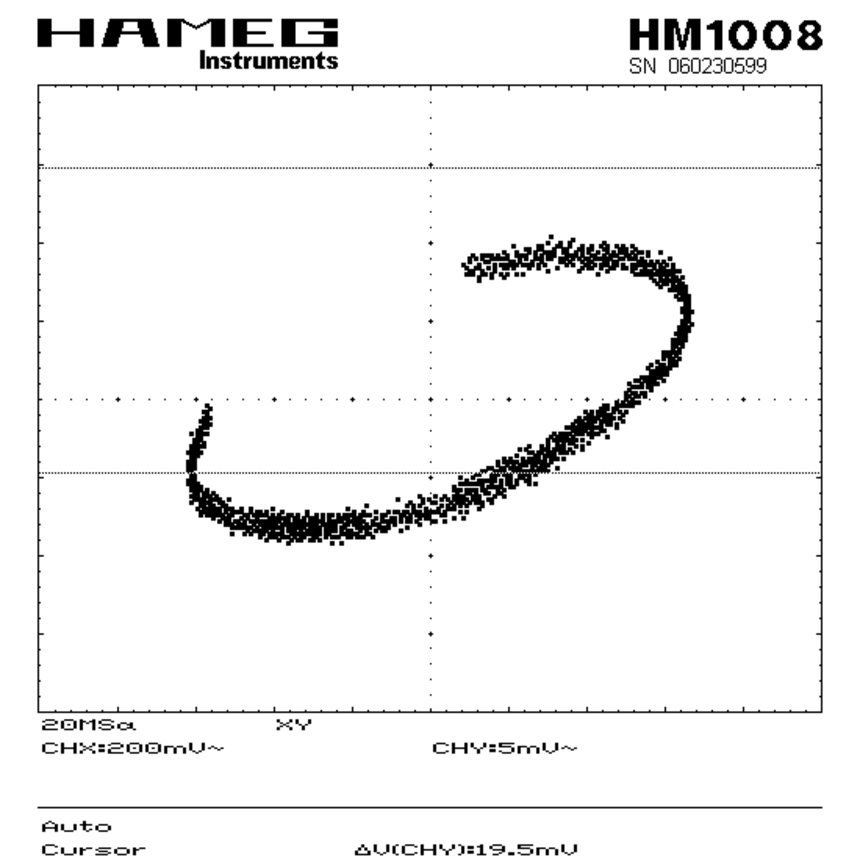
\includegraphics[width=0.4\textwidth]{img/26/Hallo_image1-72_Vergleich.pdf}
    \caption{Resonanzstellen bei 2kHz.}
    \label{fig:invarianz2}
\end{figure}

\onecolumn
\begin{figure}[!ht]
    \centering
    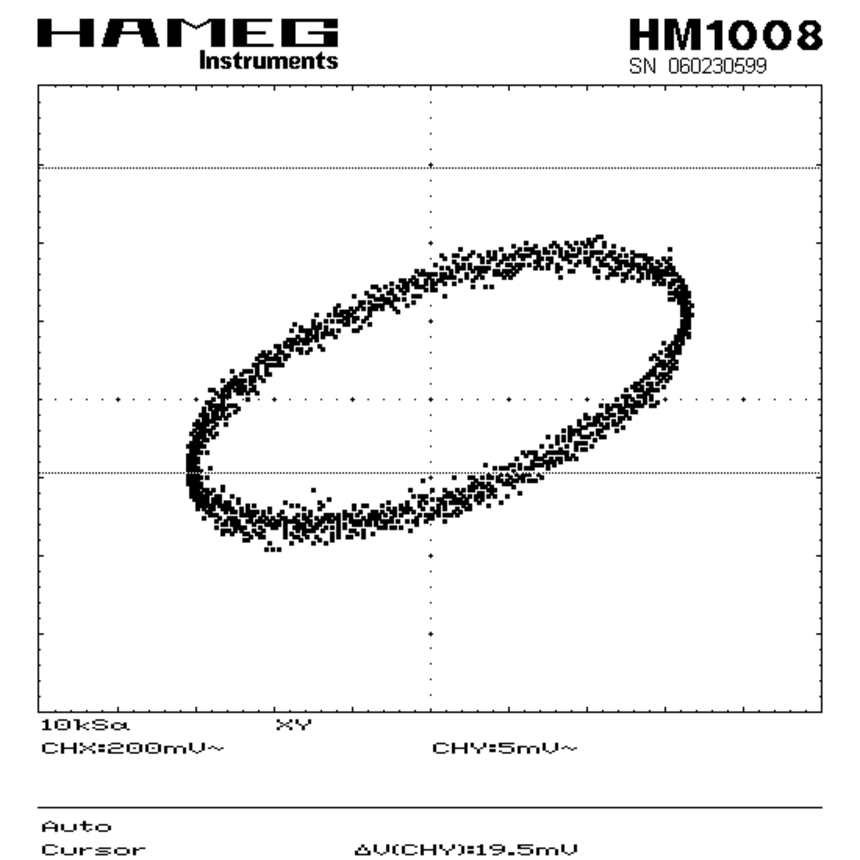
\includegraphics[width=0.45\textwidth]{img/26/Hallo_image1-6_Vergleich.pdf}
    \caption{Resonanzstellen bei 5kHz.}
    \label{fig:invarianz}
\end{figure}

\begin{figure}[!ht]
    \centering
    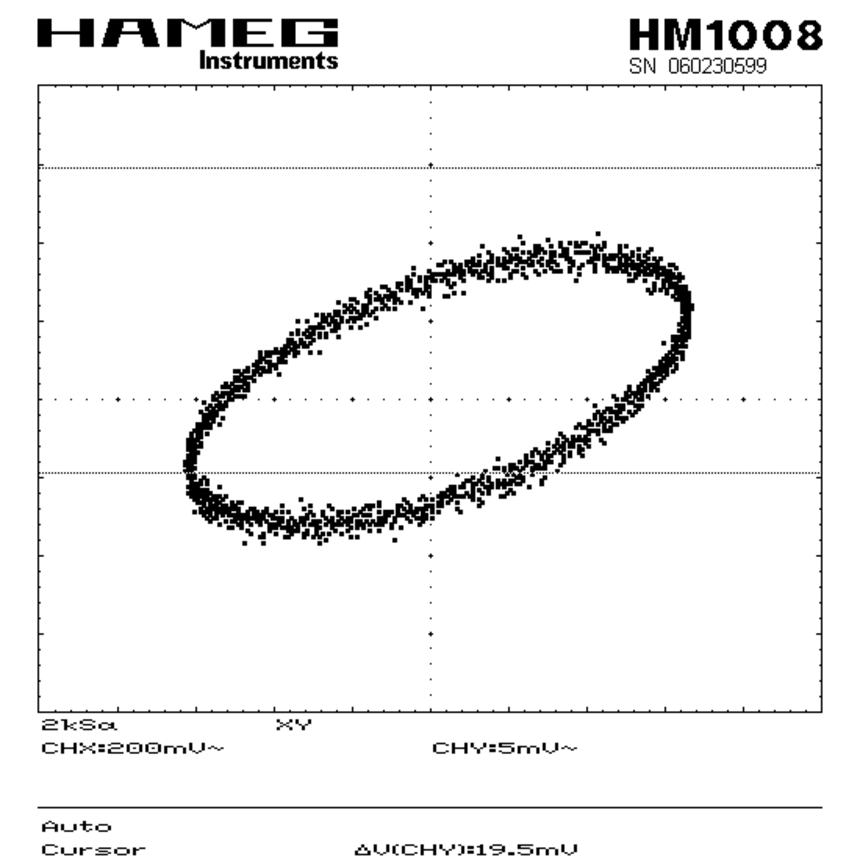
\includegraphics[width=0.45\textwidth]{img/26/Hallo_image1-7_Vergleich.pdf}
    \caption{Resonanzstellen bei 10kHz.}
    \label{fig:invarianz3}
\end{figure}
\twocolumn